\documentclass[tikz]{standalone}
\usepackage{calc}
\usepackage{amsmath}
\usepackage{amssymb}
\usepackage{amsfonts}
\usepackage{FiraSans}
\usepackage{pgf}
\definecolor{tableau1}{RGB}{31,119,180}
\definecolor{bggray}{rgb}{0.97,0.97,0.97}
\definecolor{dkgreen}{rgb}{0,0.6,0}
\definecolor{gray}{rgb}{0.75,0.75,0.75}
\definecolor{mauve}{rgb}{0.58,0,0.82}
\definecolor{backcolour}{rgb}{0.95,0.95,0.92}
\definecolor{tableau_dkblue}{RGB}{31,119,180}
\definecolor{tableau_orange}{RGB}{255,127,14}
\definecolor{tableau_dkyellow}{RGB}{139,139,0}
\definecolor{tableau_mdgreen}{RGB}{105,183,100}
\definecolor{almost_black}{RGB}{38,38,38}
\usepackage{pgfplots}
\usetikzlibrary{arrows, automata, shapes.gates.logic.US, shapes.gates.logic.IEC,
  shapes.geometric, calc, bending, shadows, backgrounds}
\pgfplotsset{
  compat={1.14},
  clip mode={individual},
  ymajorgrids={true},
  axis line style={almost_black},
  every tick/.style={almost_black},
  every axis label/.append style={almost_black},
  every tick label/.append style={almost_black},
  minor x tick style={transparent},
  tick pos={left},
  enlarge x limits={false},
  enlarge y limits={false},
  scaled x ticks={false},
  minor tick num={1},
  grid style={draw=gray!50, dashed},
  linemarkerplotopts/.style={
    mark=*, mark options={scale=1.2, solid}
  },
  lineplotopts/.style={
    no marks, color=almost_black,
    line width=1pt
  },
  scatterplotopts/.style={
    only marks, color=almost_black, mark=*,
    mark options={scale=1.2, fill=gray!70}
  }
}
\begin{document}
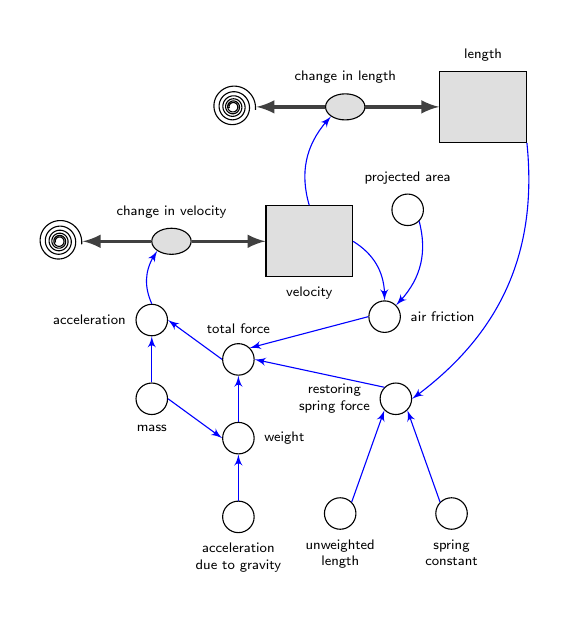
\begin{tikzpicture}
  \tikzset{background rectangle/.style={fill=white}, show background rectangle}
  \tikzstyle{stock} = [rectangle, minimum width=1.1cm, minimum height=0.9cm, text centered, draw=black, fill=gray!50]]
  \tikzstyle{flow} = [ellipse, minimum width=0.5cm, minimum height=0.15cm, text centered, draw=black, fill=gray!50]
  \tikzstyle{converter} = [circle, minimum width=0.4cm, minimum height=0.4cm, draw=black]
  \tikzstyle{spiral} = [domain=25:60, variable=\t, smooth, samples=500]
  \tikzstyle{flow-line} = [draw, very thick, color=black!75]
  \tikzstyle{line} = [draw, color=blue]
  
  \node (velocity) [stock, label={[align=center, font=\tiny\sf]below:velocity}] {};
  \node (change-in-velocity) [flow, left of=velocity, xshift=-0.75cm, label={[align=center, font=\tiny\sf]above:change in velocity}] {};
  \node (source-velocity) [left of=change-in-velocity, xshift=-0.25cm] {};

  \node (length) [stock, above right of=velocity, xshift=1.5cm, yshift=1cm, label={[align=center, font=\tiny\sf]above:length}] {};
  \node (change-in-length) [flow, left of=length, xshift=-0.75cm, label={[align=center, font=\tiny\sf]above:change in length}] {};
  \node (source-length) [left of=change-in-length, xshift=-0.25cm] {};
  
  \node (projected-area) [converter, right of=velocity, xshift=0.25cm, yshift=0.40cm, label={[align=center, font=\tiny\sf]above:projected area}] {};
  \node (air-friction) [converter, below right of=velocity, xshift=0.25cm, yshift=-0.25cm, label={[align=center, font=\tiny\sf]right:air friction}] {};
  \node (acceleration) [converter, below of=change-in-velocity, xshift=-0.25cm, label={[align=center, font=\tiny\sf]left:acceleration}] {};
  \node (mass) [converter, below of=acceleration, label={[align=center, font=\tiny\sf]below:mass}] {};
  \node (total-force) [converter, right of=acceleration, xshift=0.10cm, yshift=-0.50cm, label={[align=center, font=\tiny\sf]above:total force}] {};
  \node (weight) [converter, below of=total-force, label={[align=center, font=\tiny\sf]right:weight}] {};
  \node (acceleration-due-to-gravity) [converter, below of=weight, label={[align=center, font=\tiny\sf]below:acceleration\\due to gravity}] {};
  \node (restoring-spring-force) [converter, right of=total-force, xshift=1.00cm, yshift=-0.50cm, label={[align=center, font=\tiny\sf]left:restoring\\spring force}] {};
  \node (spring-constant) [converter, below right of=restoring-spring-force, yshift=-0.75cm, label={[align=center, font=\tiny\sf]below:spring\\constant}] {};
  \node (unweighted-length) [converter, below left of=restoring-spring-force, yshift=-0.75cm, label={[align=center, font=\tiny\sf]below:unweighted\\length}] {};
  
  \draw [spiral, shift=(source-length.west), xshift=-0.05cm] plot ({\t r}: {exp(-0.05*\t)});
  \draw [spiral, shift=(source-velocity.west), xshift=-0.05cm] plot ({\t r}: {exp(-0.05*\t)});
  
  \path [flow-line, -latex] (change-in-velocity) -- (source-velocity);
  \path [flow-line, -latex] (change-in-velocity) -- (velocity);
  \path [flow-line, -latex] (change-in-length) -- (source-length);
  \path [flow-line, -latex] (change-in-length) -- (length);
  
  \path [line] (velocity.north) edge [-latex',bend left] (change-in-length.south west);
  \path [line] (acceleration.north) edge [-latex',bend left] (change-in-velocity.south west);

  \path [line] (mass.north) edge [-latex'] (acceleration.south);
  \path [line] (total-force.west) edge [-latex'] (acceleration.east);

  \path [line] (velocity.east) edge [-latex',bend left] (air-friction.north);
  \path [line] (projected-area.south east) edge [-latex',bend left] (air-friction.north east);
  
  \path [line] (air-friction.west) edge [-latex'] (total-force.north east);
  \path [line] (weight.north) edge [-latex'] (total-force.south);
  \path [line] (restoring-spring-force.north west) edge [-latex'] (total-force.east);

  \path [line] (mass.east) edge [-latex'] (weight.west);
  \path [line] (acceleration-due-to-gravity.north) edge [-latex'] (weight.south);

  \path [line] (length.south east) edge [-latex',bend left] (restoring-spring-force.east);
  \path [line] (unweighted-length.north east) edge [-latex'] (restoring-spring-force.south west);
  \path [line] (spring-constant.north west) edge [-latex'] (restoring-spring-force.south east);
\end{tikzpicture}
\end{document}
